Due to the nature of the problem, the algorithm is separated in four different phases: the \textbf{Hotel Greedy Randomized Construction} phase, the \textbf{POI Greedy Randomized Construction} phase, the \textbf{Local Search} phase and the \textbf{Selection} phase. Some factors will be addressed before a detailed examination of each phase is viewed:
\begin{itemize}
    \item It can be seen that, unlike a normal GRASP algorithm there are two Greedy Randomized Construction phases, and this is due to the problem itself. First a GRC is done to select the initial and ending hotels of each trip, and then the second GRC is done to select the POIs in-between these hotels. This differentiation is done because it is very hard (even claimed impossible by some~\cite{divsalar2014}) to predict if a given combination of hotels will give a good solution or not.
    
    \item It can also be seen that only after the second GRC phase, Local Search is applied. This is due to the same problem addressed in the last point; since this prediction is so complicated, trying to improve a combination of hotels without knowing the score of each potential POI is wasted effort.
\end{itemize}

\subsection{Hotel Greedy Randomized Construction}
The first phase of the algorithm, contained in the $hotel\_grasp.c$ file, tries to add a starting and ending hotel to each trip minimizing the distance between the first hotel with the selected one and between the selected one with the last hotel, while trying to not break any constraint. \textit{Hotel 0} and \textit{hotel 1} represent the defined starting and finishing hotels for the tour, while the parameter $h\_rcl\_size$ given represents the size of the RCL. The pseudocode for the algorithm is the following:

\begin{algorithm}
\caption{hotel GRC}\label{euclid}
\begin{algorithmic}[1]
\State add \textit{hotel 0} as the first hotel of the first trip
\State create \textit{candidate list} with every hotel except for \textit{hotel 0}
\For{trip $t$ in trips}
\For{hotel $h$ in the candidate list}
\State $h$.score gets distance from the starting hotel to $h$ plus the distance from $h$ to \textit{hotel 1}.
\EndFor
\State sort(\textit{candidate list})
\State \textit{RCL} gets the top $h\_rcl\_size$ hotels from \textit{candidate list}.
\State \textit{selected hotel} gets hotel randomly selected from \textit{RCL}.
\State add \textit{selected hotel} to trip $t$ as its ending hotel.
\State add \textit{selected hotel} to trip $t+1$ as its starting hotel.
\EndFor
\State add \textit{hotel 1} as the ending hotel of the last trip.
\end{algorithmic}
\end{algorithm}

\newpage

\subsection{POI Greedy Randomized Construction}
The second phase of the algorithm, contained in the $poi\_grasp.c$ file, tries to add POIs to each trip, maximizing the score added while minimizing the distance added. $p\_rcl\_size$ represents the size of the RCL, and is a given parameter to the algorithm. The pseudocode for the algorithm is:

\begin{algorithm}
\caption{POI GRC}\label{euclid}
\begin{algorithmic}[1]
\State create \textit{candidate list} with every POI from the instance.
\For{trip $t$ in trips}
\While{$t$.\textit{remaining length} $\neq 0$}
\For{POI $p$ in \textit{candidate list}}
\State $p$.\textit{tmp\_score} gets $p$.\textit{score} divided by the distance added by including $p$ in $t$.
\EndFor
\State sort(\textit{candidate list})
\State \textit{RCL} gets the top $p\_rcl\_size$ POIs from \textit{candidate list}.
\State select a POI randomly from \textit{RCL} and add it to trip $t$ between the last two positions.
\EndWhile
\EndFor
\end{algorithmic}
\end{algorithm}

\subsection{Local Search and Selection}
The Local Search phase of the algorithm simply contemplates two movements selected from the best movements that can be applied to TOP according to Divsalar et al.~\cite{divsalar2013}, which are \textbf{Insert} and a variation of \textbf{Move-best} which is \textbf{In-trip Swap}. As their names sugest, the moves are fairly simple, with \textbf{Insert} trying to insert the POI which adds the highest score while adding the minimum distance into a trip, while \textbf{In-trip Swap} simply trying to swap two POIs inside one trip to improve the distance travelled in it. The amount of iterations given to the Local Search algorithm is given by the \textbf{ls\_iter\_n} parameter.

The Selection phase of the algorithm stores a tour built in the steps before if its \textbf{score} is higher than the score of the best tour found up until that iteration. It is worth noting that the algorithm repeats the whole process for a number of iterations equal to the parameter \textbf{iters\_n}.

An example of a solution built by the algorithm working on the instance $100-200-15-10.ophs$ is presented in Figure 1. The graph was made using the \textbf{visualize.py} script that can be found in the Github repository, found in Section 8.

\begin{figure}
    \centering
    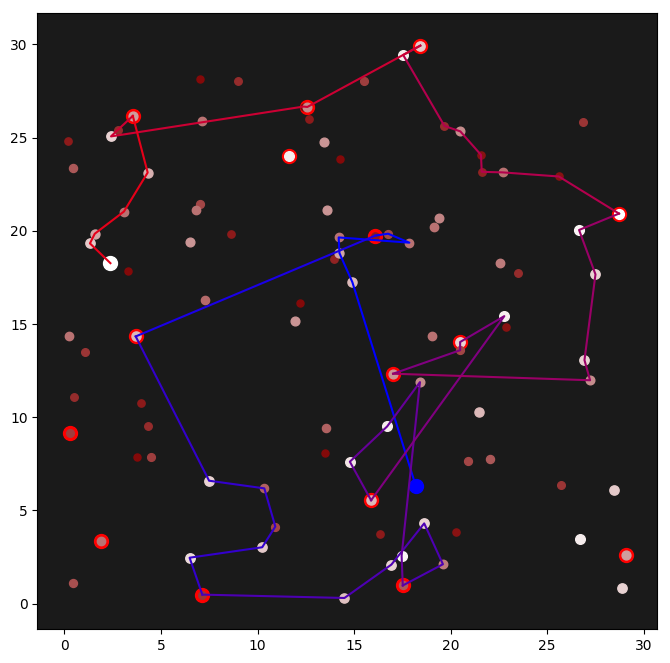
\includegraphics[width=\textwidth]{pictures/70.png}
    \caption{Example Solution: 100-200-15-10.ophsout}
    \label{fig:examplesol}
\end{figure}
